\PassOptionsToPackage{subsection=false}{beamerouterthememiniframes}
\documentclass[a4,xcolor=dvipsnames]{beamer}

\mode<presentation> {
\usetheme{Berlin}
}

\definecolor{newBlue}{HTML}{2d4457} % 2d4457 UBC Blue (primary)

\usecolortheme[named=newBlue]{structure}

\usepackage[utf8]{inputenc}
\usepackage{amsmath}
\usepackage{amsthm}
\usepackage{amssymb}
\usepackage{algorithm}
\usepackage{tikz}
\usepackage{tikz-3dplot}
\usepackage{mathtools}
\usepackage[mathscr]{euscript}
\usepackage{algpseudocode}
\usepackage{epsfig}
\usepackage{adjustbox}
\usepackage{graphicx}
\usepackage{rotating}
\usepackage{booktabs}
\usepackage{multirow}
\usepackage{subcaption}
\usepackage{multicol}
\usepackage{float}
\usepackage{hyperref}
\usepackage{wrapfig}
\usetikzlibrary{shapes.geometric, arrows.meta}

\usetikzlibrary{positioning}
\usetikzlibrary{shapes,arrows}


\def\R{\mathbb{R}}

\def\a{\mathbf{a}}
\def\b{\mathbf{b}}
\def\x{\mathbf{x}}
\def\y{\mathbf{y}}
\DeclareMathOperator*{\argmin}{argmin}
\DeclareMathOperator*{\argmax}{argmax}


\newcommand\blfootnote[1]{%
  \begingroup
  \renewcommand\thefootnote{}\footnote{#1}%
  \endgroup
}

\makeatletter
\def\blfootnote{\gdef\@thefnmark{}\@footnotetext}
\makeatother

\AtBeginSection[]{
  \begin{frame}
  \vfill
  \centering
  \begin{beamercolorbox}[sep=8pt,center,shadow=true,rounded=true]{title}
    \usebeamerfont{title}\secname\par%
  \end{beamercolorbox}
  \vfill
  \end{frame}
}


\pgfdeclarelayer{bg}    % declare background layer
\pgfsetlayers{bg,main}

\title{Machine Learning for Signal Processing}
\author{Seyyid Emre Sofuo\u{g}lu}

\begin{document}

\setlength{\leftmargini}{0.2cm}

\begin{frame}
    \titlepage
\end{frame}

\section{Introduction}
\begin{frame}
    \frametitle{Textbooks \& Resources}
    \begin{itemize}
        \item Bishop, Pattern Recognition and Machine Learning: Available in: \scriptsize{\textcolor{blue}{\href{https://www.microsoft.com/en-us/research/people/cmbishop/prml-book/}{microsoft.com/en-us/research/people/cmbishop/prml-book/}}}
        \normalsize
        \item Boyd and Vandenberghe, Introduction to Applied Linear Algebra - Vectors, Matrices, and Least Squares: \textcolor{blue}{\href{https://web.stanford.edu/~boyd/vmls/}{web.stanford.edu/\~boyd/vmls/}}
        \item Lecture slides of Mert Pilanci: \textcolor{blue}{\href{http://web.stanford.edu/class/ee269/index.html}{web.stanford.edu/class/ee269/index.html}}
        \item Too many resources online.
    \end{itemize}
\end{frame}

\begin{frame}
    \frametitle{Signal Processing}

    \begin{itemize}
        \item $x[n] = f(n)$
        \item $\mathbf{T}\left(x[n]\right) = x[n]\ast h[n] = y[n] = g(n)$.
        \item $f(n) \xrightarrow{\mathbf{T}} g(n)$.
    \end{itemize}

\end{frame}

\begin{frame}
    \frametitle{Machine Learning}
    \begin{itemize}
        \item \textbf{Wikipedia:} Machine learning (ML) is the study of computer algorithms that can improve automatically through \textbf{experience} and by the use of data.
        \item \textbf{Samuel (1959):} Field of study that gives computers
        the ability to learn without being explicitly programmed.
    \end{itemize}   
\end{frame}

\begin{frame}
    \frametitle{Why and When to use ML}
    \begin{itemize}
        \item No clear mathematical models: Cognitive recognition, language, recommendations.
        \item No fixed model: Tracking, adaptive filtering
        \item No clear math. Use data and computing power to extract the model.
    \end{itemize}
\end{frame}

\begin{frame}
    \frametitle{Types of ML}
    
    \begin{itemize}
        \item \textbf{Supervised:} Inputs (Undergrads) \textcolor{red}{$\xrightarrow{\text{Model (ECE466)}}$} targets (Signal Processing Experts).
        \item \textbf{Unsupervised:} Inputs \textcolor{red}{$\xrightarrow{Model}$ Compact representations, patterns, groups}
        \item \textbf{Self-supervised:} Pseudo-targets (supervised), from data (unsupervised).
        \item \textbf{Semi-supervised:} Weakly supervised, not all labels present.
        \item \textbf{Reinforcement learning:} No labels, carrots and sticks.
        \item Many others: Anomaly detection, dimensionality reduction, feature learning, $\ldots$.
    \end{itemize}
\end{frame}

\begin{frame}
    \frametitle{Classical Learning vs Deep Learning}
    \begin{figure}
        \centering
        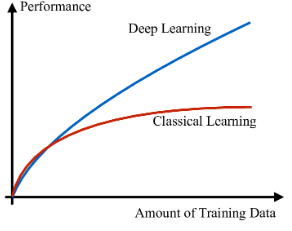
\includegraphics[width=.4\textwidth]{MLvsDL.png}
    \end{figure}
    \begin{itemize}
        \item Deep: More parameters, nonlinearity.
        \item $\uparrow$ Data, $\uparrow$ parameters, $\uparrow$ performance.
        \item Vast improvements over ML on many tasks: speech processing, natural language processing, computer vision, reinforcement learning, \ldots
    \end{itemize}
\end{frame}

\begin{frame}
    \frametitle{Summary}
    \begin{itemize}
        \item All based on optimization, linear algebra, probability, functional analysis
        \item Data vs signal?
        \item Shared tools and skillsets
        \item Directions to specialize:
        \begin{itemize}
            \item \textbf{Application:} Speech, biomedical data, recommendation systems
            \item \textbf{Theory:} Limits for models, model compression
            \item \textbf{Tools:} SWE, ML libraries, implementation and optimization procedures
            \item \textbf{Hardware:} Embedded systems, IOT, digital design
        \end{itemize}
    \end{itemize}
\end{frame}


\section{Supervised Learning}
\begin{frame}
    \frametitle{Classification}

    \begin{itemize}
        \item $x_1, x_2, x_3, \dots, x_K \in\R^{N}$, $y_1, y_2,\dots, y_K\in\{-1,1\}$.
        \item Train: $\{x\} \xrightarrow{f(.)} \{\}$.
        \item Estimate: $x_{K+1} \xrightarrow{f(.)}$ ?
    \end{itemize}
\end{frame}

\begin{frame}
    \frametitle{Binary Linear Classifier}
    \begin{gather}
        f(\x_k , \a) = f\left(\x^\top \a \right) = y_k \\
        f(c) = \begin{cases}
                1, & c\geq 0\\
                -1, & c<0
                \end{cases}
    \end{gather}
    \begin{figure}[H]
        \centering
        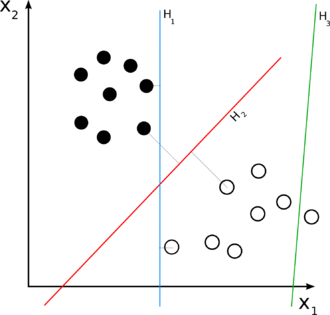
\includegraphics[width=.3\textwidth]{separating_hyperplanes.png}
    \end{figure}
\end{frame}

\begin{frame}
    \frametitle{$k$-NN Classifier}
    \begin{itemize}
        \item Class $\leftarrow$ Majority of the $k$ neighbors.
        \item Euclidean distance: $(x_{K+1}-x_{k})^2$
        \item $k=1$, nearest neighbor
        \item Good for multiple classes.
        \item Non-linear boundary, Voronoi cells
    \end{itemize}
\end{frame}
\begin{frame}
    \frametitle{Voronoi Cells}
\begin{figure}
    \centering
    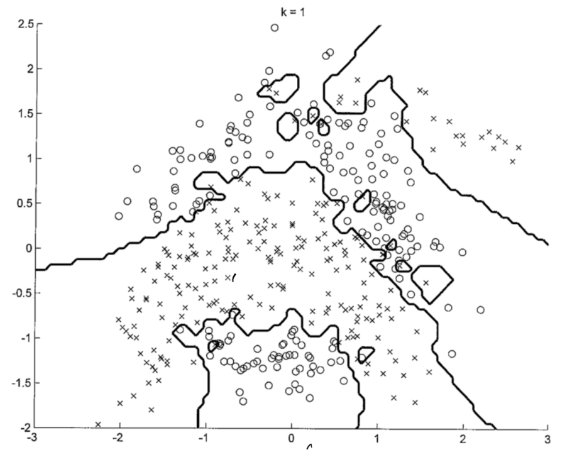
\includegraphics[width=.6\textwidth]{voronoi.png}
\end{figure}
\end{frame}

\begin{frame}
    \frametitle{Distance Measures}
    \scriptsize
\begin{itemize}
    \item $\ell_2$ distance: Euclidean.
    \item $\x_1 = [1,-1,1,\dots,1]\in\{-1,1\}^{100}$, $\x_2 = [100,0,0,0,\dots,0]\in\{0,100\}^{100}$.
    \begin{gather}
        \|\x_1-0\|_2 = 10  \qquad \|\x_2-0\|_2 = 100
    \end{gather}
    \item $\ell_1$ distance: Manhattan, absolute distance.
    \item $\|\a\|_1 = \sum_{i} |a_i|$.
    \begin{gather}
        \|x_1-0\|_2 = 100  \qquad \|x_2-0\|_2 = 100
    \end{gather}
\end{itemize}
\begin{figure}
    \centering
    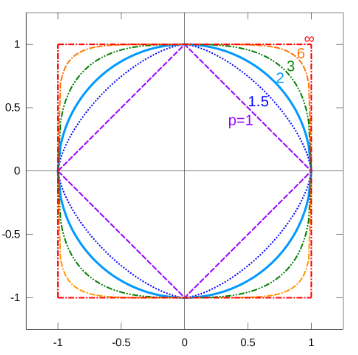
\includegraphics[width=.4\textwidth]{norms.png}
\end{figure}
\end{frame}

\begin{frame}
    \frametitle{Supervised Learning: Regression}
    $\mathbf{x} \in \mathbb{R}^N$, $\y\in \{-1,1\}^M$,
    \begin{gather}
        A\mathbf{x}+\mathbf{b} = \mathbf{y},
    \end{gather}
    variables $A\in\mathbb{R}^{M\times N}$, $\b\in\R^{M}$.
    \begin{itemize}
        \item Least squares: $(y-(ax+b))^2 \rightarrow \|\y-A\x-\b\|_2^2$.
        \item $X = [\x_1, \x_2, \x_3,\dots, \x_K]$, $Y = [\y_1, \y_2, \dots, \y_K]$ 
        \begin{align*}
            Y &= AX + \b \\
            Y &= [A, \b] [X^\top, \mathbf{1}]^\top = \hat{A} \hat{X} \\
            \hat{A} & = Y \hat{X}^{-1} \\
            \hat{A} &= Y(\hat{X}^\top\hat{X})^{-1}\hat{X}^\top 
        \end{align*}
    \end{itemize}
\end{frame}

\end{document}